\title{K-Means Parallelization \\
	Final Project Design Specification}
\author{Brian Dunlay\\
	EE590A - Winter 2017
}
\date{\today}

\documentclass[11pt]{article}
\usepackage{amsfonts}
\usepackage{mathtools}

\begin{document}
\maketitle

\section{K-Means Equations}

K-means is a clustering algorithm. Given an integer $k$ and a set of $n$ data points $X \subset \mathbb{R}^d$ we aim to choose $k$ centers $C$ so as to minimize the following function \cite{arthur}:
\newline

\begin{math}
\phi = \displaystyle\sum_{x \in X} min_{c \in C }\| x - c \|^2
\end{math}

\subsection{Iterative Algorithm}
The algorithm can be implemented in three steps:

\begin{enumerate}
\item Arbitrarily choose an initial k centers $C = {c_1, c_2, \cdots, c_k}$
\item For each $i \in {1, \cdots, k}$, set the cluster $C_i$ to be the set of points in $X$ that are closer to $c_i$ than they are to $c_j$ for all $j \neq i$
\item For each $i \in {1, \cdots, k}$, set $c_i$ to be the center of mass of all points in $C_i$: $c_i = \frac{1}{|C_i|}\sum_{x \in C_i}x$
\item Repeat Steps 2 and 3 until $C$ no longer changes
\end{enumerate}

\section{Sequential Reference}

I wrote a sequential reference in C++ in order to achieve a baseline. I found that
it is less computationally intensive to convert the image to the YUV color space and
do a comparison (euclidean distance) between points than it would have been to do
the same in RGB colorspace. 

I did not time the colorspace conversions given the fact that it is not relevant to the
immediate problem (K-Means clustering), however the conversion would be easily 
parallelizable. 

For a visual indication of the result of the k-means clustering, I colorized the clusters
based upon their mean color value along with a constant luma value. This was also omitted
from the timing of the runtime.

\subsection{Sample Image}

\begin{figure}
    \centering
    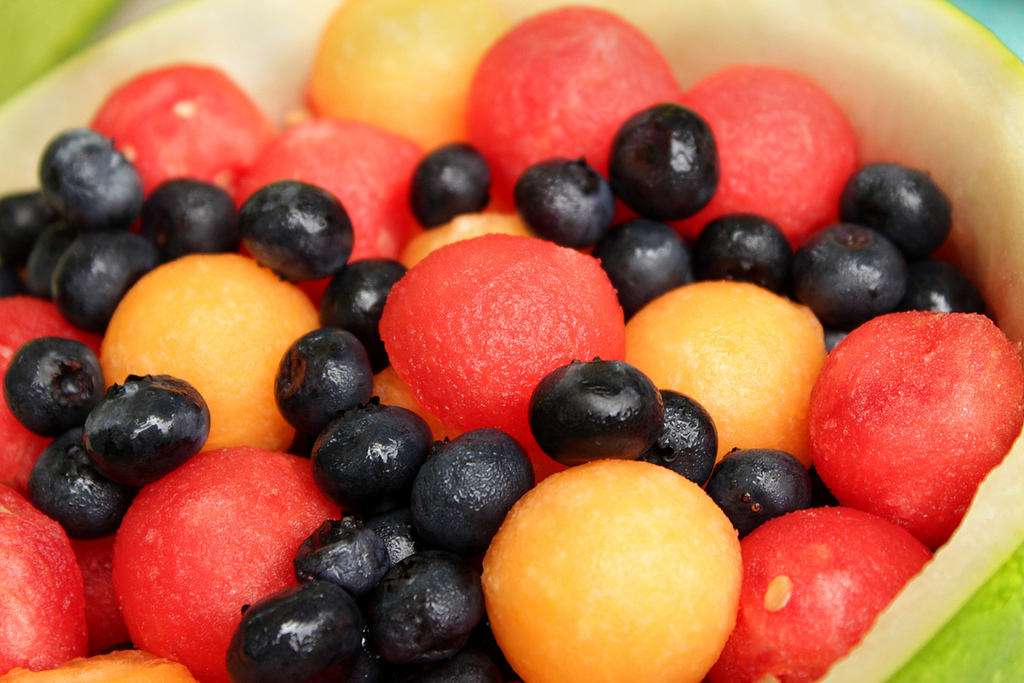
\includegraphics[width=0.6\textwidth]{fruit.png}
    \caption{Image\cite{fruit} before segmentation}
    \label{fig:fruit}
\end{figure}

\begin{figure}
    \centering
    
\includegraphics[width=0.6\textwidth]{fruit-segmented.png}
    \caption{Image after segmentation}
    \label{fig:fruit-segmented}
\end{figure}

This image was segmented based on 5 coordinates that were hand-picked as input to the program.
The average runtime over 30 runs for processing this image was 3.026 seconds. 

\subsection{Code}

See \emph{sequential-kmeans.cpp} for the sequential code reference implementation.

\section{Complexity Analysis}

\section{Parallel Pseudo-Code}

See \emph{parallel-kmeans.cl} for the parallel pseudo-code implementation.


\begin{thebibliography}{9}

\bibitem{arthur}
  David Arthur and Sergei Vassilvitskii,
  \emph{k-means++: The Advantages of Careful Seeding},
  http://ilpubs.stanford.edu:8090/778/1/2006-13.pdf

\bibitem{fruit}
  Didriks,
  Fruit Salad,
  https://flic.kr/p/a6W1Te

\end{thebibliography}

\end{document}
This is never printed
